\subsection{What is Function-Fiasco}
\begin{frame}
  \frametitle{What is Function-Fiasco}
    \begin{center}
      \huge{\textbf{A Pseudo-tested method detection tool}}

      
\includegraphics[scale = .15]{images/wrench}
    \end{center}
\end{frame}

\subsection{Flow}
\begin{frame}
  \frametitle{Flow to system}
    \begin{center}
      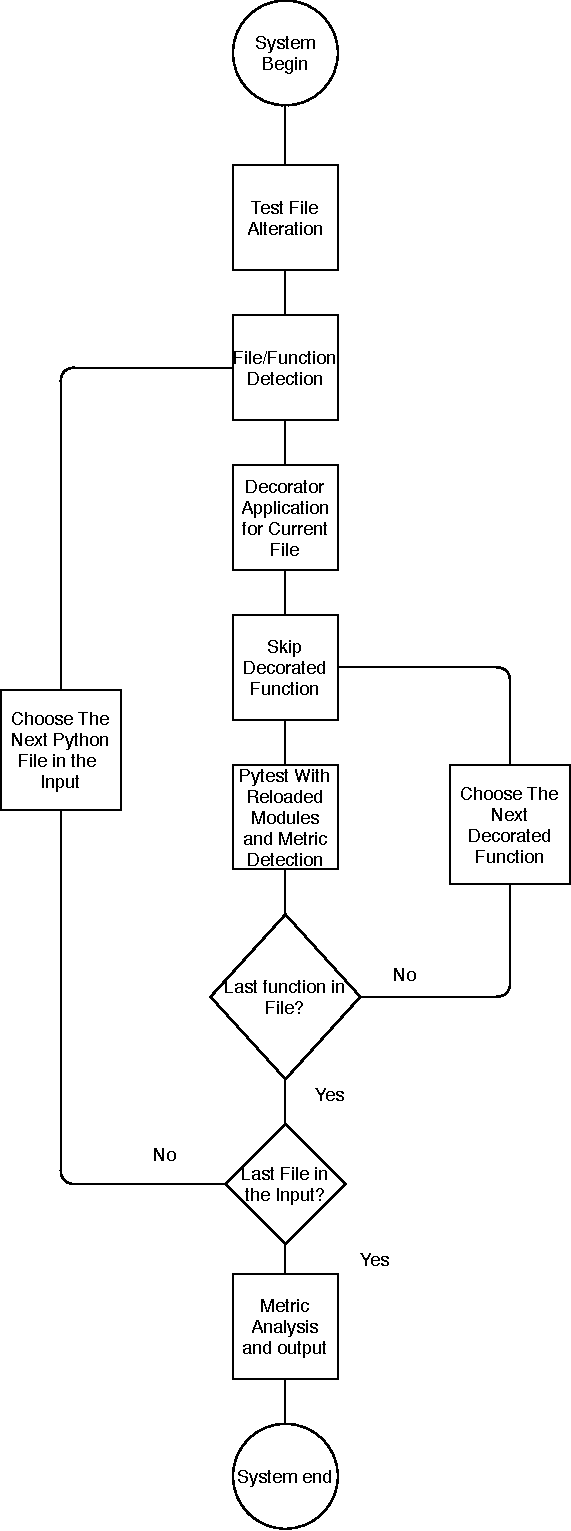
\includegraphics[scale = .25]{images/flow1}
    \end{center}
\end{frame}

\begin{frame}
  \frametitle{Beginning}
  \begin{center}
    
\includegraphics[scale = .5]{images/beginning}
  \end{center}
\end{frame}

\begin{frame}[fragile]
  \frametitle{Reloader Function}
  \begin{figure}[t!, scale = .75]
	\begin{lstlisting}[language = Python, basicstyle=\small, backgroundcolor = \color{lightgray}]
 def reloader():
   for modules in listToReload:
     importlib.reload(modules)
\end{lstlisting}
  \end{figure}
\end{frame}

\begin{frame}
  \frametitle{Next Steps}
  \begin{center}
    
\includegraphics[scale = .5]{images/second}
  \end{center}
\end{frame}

\begin{frame}[fragile]
  \frametitle{Decorator Function}
  \begin{figure}[t!, scale = .75]
	\begin{lstlisting}[language = Python, basicstyle=\small, backgroundcolor = \color{lightgray}]
  def skipper(func):
    if(func.__name__ in functionsComplete):
      def doFunc(*args, **kwargs):
        return 5
      return doFunc

    else:
      def doFunc(*args, **kwargs):
        var = func(*args, **kwargs)
          return var
      return doFunc
  \end{lstlisting}
\end{figure}
\end{frame}

\begin{frame}
  \frametitle{Pytesting}
  \begin{center}
    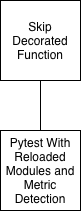
\includegraphics[scale = .5]{images/decoration}
  \end{center}
\end{frame}

\begin{frame}
  \frametitle{File and Function Checks}
  \begin{center}
    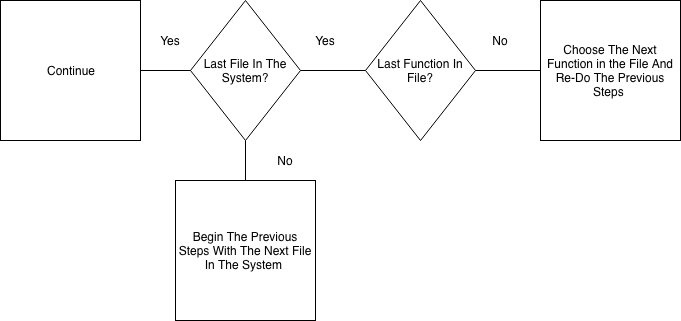
\includegraphics[scale = .35]{images/decisions}
  \end{center}
\end{frame}

\begin{frame}
  \frametitle{System End}
  \begin{center}
    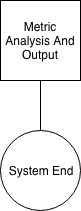
\includegraphics[scale = .5]{images/systemEnd}
  \end{center}
\end{frame}
